% ============================================================================
\section{Characterization of 2-planar graphs}
\label{sec:2planar}
% ============================================================================

Let $G$ be an optimal $2$-planar graph on $n$ vertices (and therefore with $5n-10$ edges). Let also $\Gamma(G)$ be a PMCM $2$-planar drawing of $G$, i.e. $\Gamma(G)$ has the maximum number of true-planar edges among all potential $2$-planar drawing of $G$ and, subject to this restriction, $\Gamma(G)$ has also the minimum number of crossings. For the sake of simplicity we also momentarily assume that in $\Gamma(G)$ there is no pair of edges that cross twice, i.e. $\Gamma(G)$ is almost-simple. This assumption  will be settled soon (see Lemma~\ref{lem:2_planar_cross_twice}). In the following lemmas, we examine structural properties of an almost-simple PMCM-drawing $\Gamma(G)$.

Note that in an almost-simple PMCM-drawing $\Gamma(G)$, whenever edge $(w,w')$ has at least $2$ crossings, say $c$ and $c'$, then there exist two (non identical) edges $(u,u')$ and $(v,v')$ that cross $(w,w')$ at $c$ and $c'$ respectively. This implies that vertices $u$ and $v$ always form a parallel pair, and so do vertices $u'$ and $v'$. Since this property will be heavily used throughout the paper, we shall not explicitly state it every time, but rather implicitly imply it.

%\todo[inline]{add in every lemma the assumption about edges crossing twice}

\begin{lemma}
Let $\Gamma(G)$ be an almost-simple PMCM $2$-planar drawing of an optimal $2$-planar graph $G$ on $n$ vertices. Any edge that is crossed twice in  $\Gamma(G)$ is a chord of a true-planar $5$-cycle in $\Gamma(G)$. 
\label{lem:2_planar_small_faces}
\end{lemma}

\begin{proof}
Let $(w,w')$ be an edge of $G$ that is crossed twice in $\Gamma(G)$ and let $(u,u')$ and $(v,v')$ be the corresponding edges crossed by $(w,w')$. This crossing configuration defines four corner pairs: $\{w,u\}$, $\{w,u'\}$, $\{w,v\}$, $\{w,v'\}$, and two parallel pairs: $\{u,v\}$ and $\{u',v'\}$. By Lemmas~\ref{lem:crossing_twice} and ~\ref{lem:crossing_adjacent}, all corner edges are \pes, and either one or two of the parallel edges are \pes. We distinguish two cases depending on whether both parallel edges are \pes or not.

%Let $(u,v)$ be an edge of $G$ that is crossed twice in $\Gamma(G)$ and let $(u_1,v_1)$ and $(u_2,v_2)$ be the corresponding edges crossed by $(u,v)$. This crossing configuration defines four corner pairs: $\{u,u_1\}$, $\{u,v_1\}$, $\{v,u_2\}$, $\{v,v_2\}$, and two parallel pairs: $\{u_1,u_2\}$ and $\{v_1,v_2\}$. By P.\ref{prop_corner} and P.\ref{prop_parallel}, all the potential corner edges exist, and there exists either one or two of the potential parallel edges. We distinguish two cases depending on whether there exist both potential parallel edges or not.

So suppose first, that both parallel edges $(u,v)$ and $(u',v')$ are \pes, as in Figure~\ref{fig:2_planar_both_parallel_before}. Then vertices $w,u,v,w',v',u'$ define a \pp $\mathcal{P}_6$ of six vertices (grey shaded in Figure~\ref{fig:2_planar_both_parallel_before}). The \pr $\mathcal{R}_6$ of $\mathcal{P}_6$ contains no vertices in its interior, and at most five edges of $\Gamma(G)$ pass through $\mathcal{R}_6$: edges $(w,w')$, $(u,u')$, $(v,v')$ and at most two other edges that cross $(u,u')$ or $(v,v')$. Note that since the \pr is an open topological region without vertices in its interior, there can not be an edge that lies entirely in its interior. We proceed by removing  edges $(w,w')$, $(u,u')$, $(v,v')$ and all other edges that cross $(u,u')$ or $(v,v')$, and replace them with the $2$-planar pattern of Figure~\ref{fig:2_planar_both_parallel_after}. In the derived graph there exist $6$ edges drawn in $\mathcal{R}_6$ and do not cross the boundary of the \pp. Hence, the derived graph has more edges than $G$; a contradiction to the optimality of $G$. Note that even in the case where the \pp is not simple, i.e. the vertices that define its boundary are not all distinct, the above argument still holds, as can be seen for example in Figure~\ref{fig:2_planar_both_parallel_non_simple}, where $w=u$ and $v=v'$.
\todo{fix the figure}
%So suppose first, that both potential parallel edges $(u_1,u_2)$ and $(v_1,v_2)$ exist, as in Figure~\ref{fig:2_planar_both_parallel_before}. Then vertices $u,u_1,u_2,v,v_2,v_1$ define a \pp $\mathcal{P}_6$ of six vertices (grey shaded in Figure~\ref{fig:2_planar_both_parallel_before}). The polygonal region $\mathcal{R}_6$ of $\mathcal{P}_6$ contains no vertices in its interior, and at most five edges of $\Gamma(G)$ pass through $\mathcal{R}_6$: edges $(u,v)$, $(u_1,v_1)$, $(u_2,v_2)$ and at most two other edges that cross $(u_1,v_1)$ or $(u_2,v_2)$. Note that since the polygonal region is an open topological region without vertices in its interior, there can not be an edge that lies entirely in its interior. We proceed by removing  edges $(u,v)$, $(u_1,v_1)$, $(u_2,v_2)$ and all other edges that cross $(u_1,v_1)$ or $(u_2,v_2)$, and replace them with the $2$-planar pattern of Figure~\ref{fig:2_planar_both_parallel_after}. In the derived graph there exist $6$ edges drawn in $\mathcal{R}_6$ and do not cross the boundary of the \pp. Hence, the derived graph has more edges than $G$; a contradiction to the optimality of $G$. Note that even in the case where the \pp is not simple, i.e. the vertices that define its boundary are not all distinct, the above argument still holds, as can be seen for example in Figure~\ref{fig:2_planar_both_parallel_non_simple}, where $u=u_1$ and $v_1=v_2$.

Suppose now that parallel edge $(u,v)$ is not a \pe. Then, it is $u=v$; refer to Figure~\ref{fig:2_planar_one_parallel_before}. This time, vertices $w,u,w',v',u'$ define a \pp $\mathcal{P}_5$ of five vertices (grey shaded in Figure~\ref{fig:2_planar_one_parallel_before}). As in the previous case, at most five edges of $\Gamma(G)$ pass through the polygonal region $\mathcal{R}_5$. We proceed by removing  edges $(w,w')$, $(u,u')$, $(v,v')$ and all other edges that cross $(u,u')$ or $(v,v')$, and replace them with the $2$-planar pattern of Figure~\ref{fig:2_planar_one_parallel_after}. In the derived graph there exist $5$ edges drawn in $\mathcal{R}_5$ plus the five \pes of the boundary of $\mathcal{P}_5$. Since $G$ is optimal, it follows that:
\begin{enumerate}
\item there exist exactly two edges other than $(w,w')$, say $e_1$ and $e_2$, that cross $(u,v)$ and $(u',v')$ respectively, and
\item  the \pes of the boundary of  $\mathcal{P}_5$ already exist in the drawing $\Gamma(G)$, i.e. $\mathcal{P}_5$ is a cycle, say $C$, of length $5$. 
\end{enumerate}

%Suppose now that potential parallel edge $(u_1,u_2)$ does not exist. Then, it is $u_1=u_2$; refer to Figure~\ref{fig:2_planar_one_parallel_before}. This time, vertices $u,u_1,v,v_2,v_1$ define a \pp $\mathcal{P}_5$ of five vertices (grey shaded in Figure~\ref{fig:2_planar_one_parallel_before}). As in the previous case, at most five edges of $\Gamma(G)$ pass through the polygonal region $\mathcal{R}_5$. We proceed by removing  edges $(u,v)$, $(u_1,v_1)$, $(u_1,v_2)$ and all other edges that cross $(u_1,v_1)$ or $(u_2,v_2)$, and replace them with the $2$-planar pattern of Figure~\ref{fig:2_planar_one_parallel_after}. In the derived graph there exist $5$ edges drawn in $\mathcal{R}_5$ plus the five \pes of the boundary of $\mathcal{P}_5$. Since $G$ is optimal, it follows that:
%\begin{enumerate}
%\item there exist exactly two edges other than $(u,v)$, say $e_1$ and $e_2$, that cross $(u_1,v_1)$ and $(u_1,v_2)$ respectively, and
%\item  the \pes of the boundary of  $\mathcal{P}_5$ already exist in the drawing $\Gamma(G)$, i.e. $\mathcal{P}_5$ is a cycle, say $C$, of length $5$. 
%\end{enumerate}

If $C$ is a true-planar $5$-cycle in $\Gamma(G)$ the lemma holds, so suppose that this is not the case. Then, at least one of edges $e_1$ or $e_2$ crosses $C$. Suppose w.l.o.g. that  edge $e_1=(w_1,w'_1)$ crosses edge $(v,v')$ of the $5$-cycle $C$ at crossing point $c$ (the case where $e_1$ crosses edge $(u,v)$ can be treated similarly);\todo{is it clear that it can't cross another edge of C?} refer to Figure~\ref{fig:2_planar_one_parallel_extra}. Note that $e_1$ already has two crossings in the drawing $\Gamma(G)$. Then, at least one of the edge segments $(w_1,c)$ or $(c,w'_1)$ of $e_1$ does not pass through the \pr $\mathcal{R}_5$. Suppose w.l.o.g. that this is edge segment $(w_1,c)$  of $e_1$. Then, vertices $w_1$ - $v$, and $w_1$ - $v'$ define two corner pairs of vertices. Hence vertices $w,u,w',v',w_1,v$ define a \pp $\mathcal{P}_6$ on six vertices, with exactly six edges passing through its \pr, say $\mathcal{R}_6$. We remove all edges that pass through $\mathcal{R}_6$ and replace it with the $2$-planar pattern of Figure~\ref{fig:2_planar_one_parallel_final}: we add one vertex and a total of $12$ edges. The derived graph, say $G'$, is $2$-planar and has $n'=n+1$ vertices and $m'=m+6$ edges (where $n$, $m$ are the number of vertices and edges of $G$ respectively). Hence $m'=5n'-9>5n'-10$, i.e. $G'$ has more edges than allowed; a contradiction.

%If $C$ is a true-planar $5$-cycle in $\Gamma(G)$ the lemma holds, so suppose that this is not the case. Then, at least one of edges $e_1$ or $e_2$ crosses $C$. Suppose w.l.o.g. that  edge $e_1=(w,w')$ crosses edge $(v_1,v_2)$ of the $5$-cycle $C$ at crossing point $c$ (the case where $e_1$ crosses edge $(u,v_1)$ can be treated similarly);\todo{is it clear that it can't cross another edge of C?} refer to Figure~\ref{fig:2_planar_one_parallel_extra}. Note that $e_1$ already has two crossings in the drawing $\Gamma(G)$. Then, at least one of the edge segments $(w,c)$ or $(c,w')$ of $e_1$ does not pass through the polygonal region $\mathcal{R}_5$. Suppose w.l.o.g. that this is edge segment $(w,c)$  of $e_1$. Then, vertices $w$ - $v_1$, and $w$ - $v_2$ define two corner pairs of vertices. Hence vertices $u,u_1,v,v_2,w,v_1$ define a polygonal region $\mathcal{P}_6$ on six vertices, with exactly six edges passing through its polygonal region, say $\mathcal{R}_6$. We remove all edges that pass through $\mathcal{R}_6$ and replace it with the $2$-planar pattern of Figure~\ref{fig:2_planar_one_parallel_final}: we add one vertex and a total of $12$ edges. The derived graph, say $G'$, is $2$-planar and has $n'=n+1$ vertices and $m'=m+6$ edges (where $n$, $m$ are the number of vertices and edges of $G$ respectively). Hence $m'=5n'-9>5n'-10$, i.e. $G'$ has more edges than allowed; a contradiction.\qed
\end{proof}

\begin{figure}[htb]
    \centering
    \begin{minipage}[b]{.24\textwidth}
        \centering
        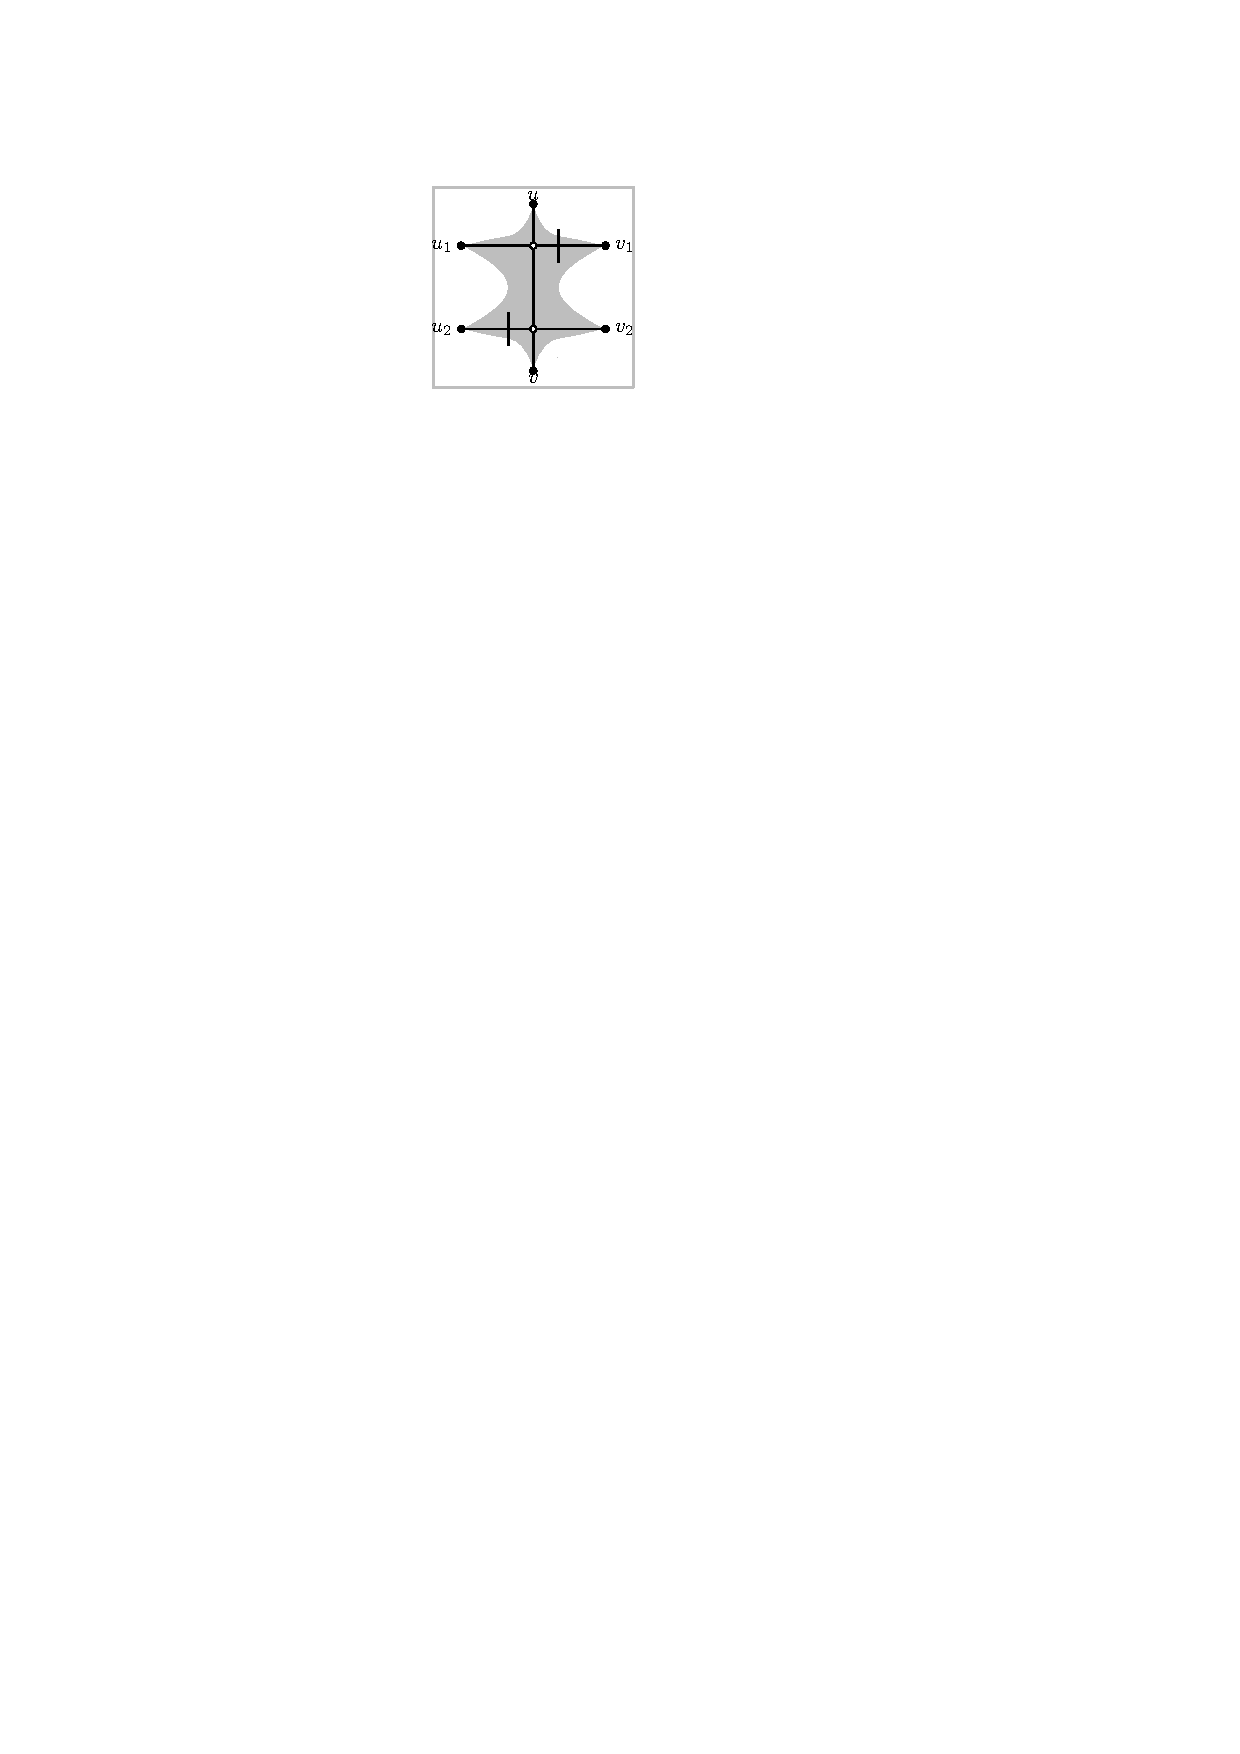
\includegraphics[width=\textwidth,page=1]{images/2_planar_potential_parallel}
        \subcaption{~}\label{fig:2_planar_both_parallel_before}
    \end{minipage}
    \begin{minipage}[b]{.24\textwidth}
        \centering
        \includegraphics[width=\textwidth,page=2]{images/2_planar_potential_parallel}
        \subcaption{~}\label{fig:2_planar_both_parallel_after}
    \end{minipage}
	\begin{minipage}[b]{.24\textwidth}
        \centering        
        \includegraphics[width=\textwidth,page=3]{images/2_planar_potential_parallel}
        \subcaption{~}\label{fig:2_planar_both_parallel_non_simple}
    \end{minipage}
		
    \begin{minipage}[b]{.24\textwidth}
        \centering
        \includegraphics[width=\textwidth,page=4]{images/2_planar_potential_parallel}
        \subcaption{~}\label{fig:2_planar_one_parallel_before}
    \end{minipage}
		\begin{minipage}[b]{.24\textwidth}
        \centering
        \includegraphics[width=\textwidth,page=5]{images/2_planar_potential_parallel}
        \subcaption{~}\label{fig:2_planar_one_parallel_after}
    \end{minipage}
		\begin{minipage}[b]{.24\textwidth}
        \centering
        \includegraphics[width=\textwidth,page=6]{images/2_planar_potential_parallel}
        \subcaption{~}\label{fig:2_planar_one_parallel_extra}
    \end{minipage}
		\begin{minipage}[b]{.24\textwidth}
        \centering
        \includegraphics[width=\textwidth,page=7]{images/2_planar_potential_parallel}
        \subcaption{~}\label{fig:2_planar_one_parallel_final}
    \end{minipage}
    \caption{%
    Different configurations used in Lemma~\ref{lem:2_planar_small_faces}.}
    \label{fig:2_planar_potential_parallel}
\end{figure}




By Lemma~\ref{lem:2_planar_small_faces}, we have that any edge of $G$ that is crossed twice in an almost-simple PMCM-drawing $\Gamma(G)$ is a chord of a true-planar $5$-cycle. So, it remains to consider edges of $G$ that have only one crossing in $\Gamma(G)$:

\begin{lemma}\label{lem:2_planar_one_crossing}
Let $\Gamma(G)$ be an almost-simple PMCM $2$-planar drawing of an optimal $2$-planar graph $G$ on $n$ vertices. Then every edge of $\Gamma(G)$ is either true-planar or has exactly two crossings.
\end{lemma}
\begin{proof}
By the proof of Lemma~\ref{lem:2_planar_small_faces}, we have that, for any edge of $G$ that is crossed twice in $\Gamma(G)$, both edges that cross this particular edge also have two crossing in $\Gamma(G)$. This implies that if edges $(u,u')$ and $(v,v')$ cross in $\Gamma(G)$ and $(u,u')$ has only one crossing, then the same holds for $(v,v')$. \todo{use propagated set}So, we have four corner pairs of  vertices: $u$ - $v$, $u$ - $v'$, $u'$ - $v$, $u'$ - $v'$, and all corner edges are \pes; refer to Figure~\ref{fig:2_planar_one_crossing_before}. Vertices  $u,v,v',u'$ define a \pp $\mathcal{P}_4$ of four vertices (grey shaded in Figure~\ref{fig:2_planar_one_crossing_before}). Since edges $(u,u')$ and $(v,v')$ have only one crossing each, the \pes of the boundary of $\mathcal{P}_4$ exist in $\Gamma(G)$ and are true-planar edges (Indeed if any of these \pes does not exist, one could add them in $\Gamma(G)$ without introducing any crossings or creating homotopic edges, contradicting the optimality of $G$). We proceed by removing  edges $(u,u')$ and $(v,v')$, and replace them with the $2$-planar pattern of Figure~\ref{fig:2_planar_one_crossing_after}. The derived graph, say $G'$ is $2$-planar and has $n'=n+2$ vertices and $m'=m+11$ edges (where $n$, $m$ are the number of vertices and edges of $G$ respectively). Hence $m'=5n'-9>5n'-10$, i.e. $G'$ has more edges than allowed; a contradiction.

%By the proof of Lemma~\ref{lem:2_planar_small_faces}, we have that, for any edge of $G$ that is crossed twice in $\Gamma(G)$, both edges that cross this particular edge also have two crossing in $\Gamma(G)$. This implies that if edges $(u_1,v_1)$ and $(u_2,v_2)$ cross in $\Gamma(G)$ and $(u_1,v_1)$ has only one crossing, then the same holds for $(u_2,v_2)$. So, we have four corner pairs of  vertices: $u_1$ - $u_2$, $u_1$ - $v_2$, $v_1$ - $u_2$, $v_1$ - $v_2$, and all the potential corner edges exist; refer to Figure~\ref{fig:2_planar_one_crossing_before}. Vertices  $u_1,u_2,v_2,v_1$ define a \pp $\mathcal{P}_4$ of four vertices (grey shaded in Figure~\ref{fig:2_planar_one_crossing_before}). Since edges $(u_1,v_1)$ and $(u_2,v_2)$ have only one crossing each, the \pes of the boundary of $\mathcal{P}_4$ exist in $\Gamma(G)$ and are true-planar edges (Indeed if any of these \pes does not exist, one could add them in $\Gamma(G)$ without introducing any crossings or creating homotopic edges, contradicting the optimality of $G$). We proceed by removing  edges $(u_1,v_1)$ and $(u_2,v_2)$, and replace them with the $2$-planar pattern of Figure~\ref{fig:2_planar_one_crossing_after}. The derived graph, say $G'$ is $2$-planar and has $n'=n+2$ vertices and $m'=m+11$ edges (where $n$, $m$ are the number of vertices and edges of $G$ respectively). Hence $m'=5n'-9>5n'-10$, i.e. $G'$ has more edges than allowed; a contradiction.\qed
\end{proof}


\begin{figure}[htb]
    \centering
    \begin{minipage}[b]{.24\textwidth}
        \centering
        
\includegraphics[width=\textwidth,page=1]{images/2planar_one_crossing}
        \subcaption{~}\label{fig:2_planar_one_crossing_before}
    \end{minipage}
    \begin{minipage}[b]{.24\textwidth}
        \centering
        
\includegraphics[width=\textwidth,page=2]{images/2planar_one_crossing}
        \subcaption{~}\label{fig:2_planar_one_crossing_after}
    \end{minipage}
    \caption{%
    Configurations used in Lemma~\ref{lem:2_planar_one_crossing}}.
    \label{fig:2_planar_one_crossing}
\end{figure}

almost-simple PMCM
 
Now we are ready to prove the main property of every almost-simple PMCM-drawing $\Gamma(G)$ of a maximal $2$-planar graph. By Lemmas~\ref{lem:2_planar_small_faces} and \ref{lem:2_planar_one_crossing} we have that there exist only edges with two crossings and true-planar edges in $\Gamma(G)$ that create only true-planar $5$-cycles. Hence we have proven the following:
 
 %\todo[inline]{make lemma~\ref{lem:2_planar_faces} a corrolary}
 \begin{corollary}\label{cor:2_planar_faces}
  The true planar skeleton $\Pi(G)$ of an almost-simple PMCM-drawing $\Gamma(G)$ of a maximal $2$-planar graph $G$ contains only faces of length $5$.
 \end{corollary}
 %Now we are ready to prove the main property of maximal $2$-planar graphs. By Lemmas~\ref{lem:2_planar_small_faces} and \ref{lem:2_planar_one_crossing} we have that there exist only edges with two crossings and true-planar edges in $\Gamma(G)$ that create only $5$-cycles. Hence we have proven the following:
 %
 %\todo[inline]{make lemma~\ref{lem:2_planar_faces} a corrolary}
 %\begin{lemma}\label{lem:2_planar_faces}
  %The true planar subgraph $G_p$\todo{do we use true planar subgraph as notation?} contains only faces of length $5$.
 %\end{lemma}

Recall that at the beginning of this section we made the assumption that there is no pair of edges that cross twice in the drawing $\Gamma(G)$, i.e. that $\Gamma(G)$ is almost-simple. In the following, we prove that any PMCM-drawing of a maximal $2$-planar graph is almost-simple.
%Recall that at the beginning of this section we made the assumption that there is no pair of edges that cross twice in the drawing $\Gamma(G)$. In the following, we prove that in a planar-maximal crossing-minimal drawing there are no such pairs of edges.



%\begin{lemma}
%Let $\Gamma(G)$ be a $2$-planar drawing of an optimal $2$-planar graph $G$ on $n$ vertices. There is no pair of edges that cross twice in $\Gamma(G)$. 
%\label{lem:2_planar_cross_twice}
%\end{lemma}
%
%\begin{proof}
%Suppose that there exist edges $(u_1,v_1)$ and $(u_2,v_2)$ that cross twice at crossing points $c_1$ and $c_2$. Consider the bounded region $R$ defined by $(c_1,c_2)$ segment of edges $(u_1,v_1)$ and $(u_2,v_2)$. Since edges $(u_1,v_1)$ and $(u_2,v_2)$ both have two crossings, no other edge of $G$ crosses the boundary of $R$. Hence, if there exists at least one vertex of $G$ inside this region, $G$ is not connected; a contradiction.\todo{mention that G is connected} On the other hand, if $R$ is empty, we could redraw edges $(u_1,v_1)$ and $(u_2,v_2)$ so that they do not cross; a contradiction to the fact that $\Gamma(G)$ is crossing-minimal.\qed
%\end{proof}

By combining Lemmas~\ref{lem:2_planar_faces} and \ref{lem:2_planar_cross_twice}, we can characterize all optimal $2$-planar graphs:


 By Lemma~\ref{lem:2_planar_cross_twice} we have that Lemma~\ref{lem:2_planar_faces} holds for all maximal $2$-planar graphs. Since the true planar skeleton of such a graph contains only faces of length $5$, we can start with a $5$-tiling of the plane\todo{rephrase}. Now in the interior of every face of length $5$, we can add all  $5$ missing edges using the $2$-planar pattern of Figure~\ref{fig:2_planar_one_parallel_after}.

